\documentclass[hints, space]{ximera}
%% handout
%% space
%% newpage
%% numbers
%% nooutcomes

%I added the commands here so that I would't have to keep looking them up
%\newcommand{\RR}{\mathbb R}
%\renewcommand{\d}{\,d}
%\newcommand{\dd}[2][]{\frac{d #1}{d #2}}
%\renewcommand{\l}{\ell}
%\newcommand{\ddx}{\frac{d}{dx}}
%\everymath{\displaystyle}
%\newcommand{\dfn}{\textbf}
%\newcommand{\eval}[1]{\bigg[ #1 \bigg]}

%\begin{image}
%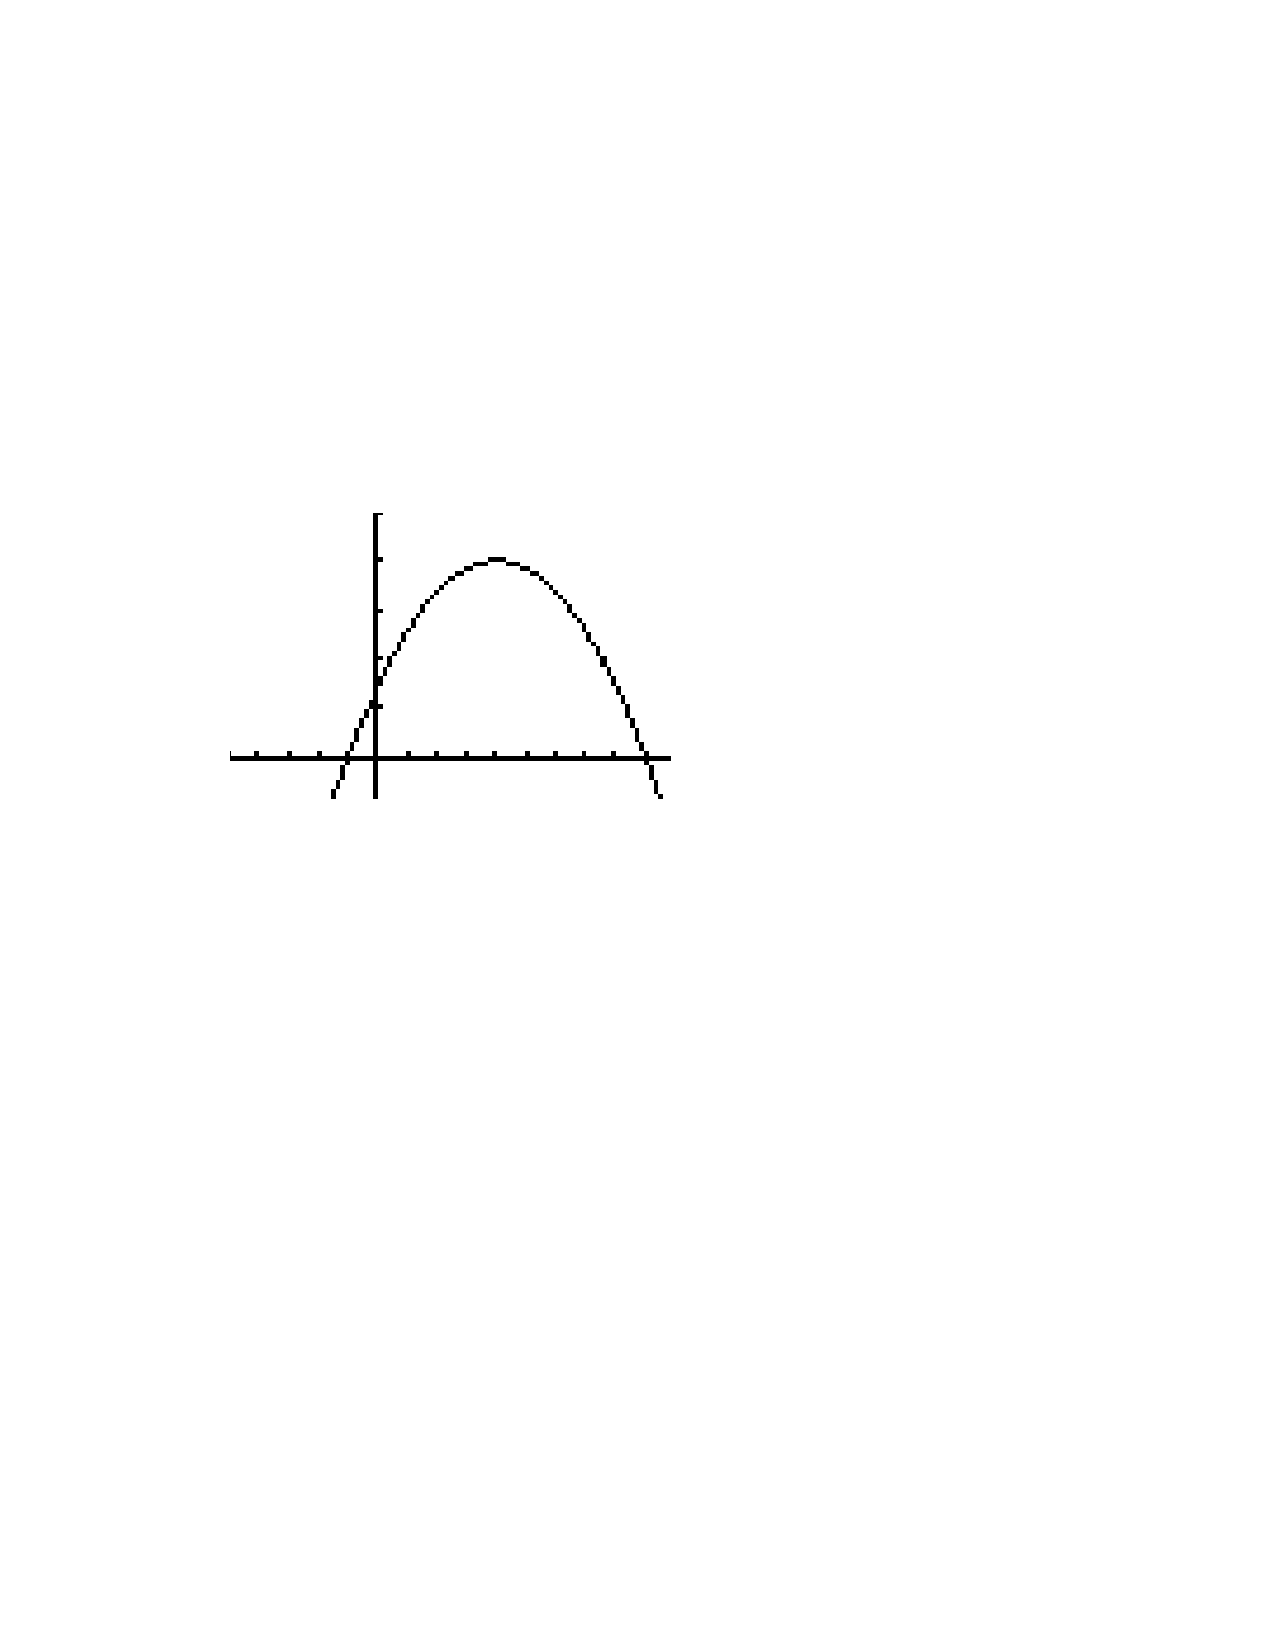
\includegraphics[trim= 170 420 250 180]{Figure1.pdf}
%\end{image}




\title{Recitation \#27 - 5.5 Substitution Rule}  

\begin{document}
\begin{abstract}    more practice		\end{abstract}
\maketitle

Dummy Latex file


\begin{question}
What is the largest prime number?
	\begin{hint}
	This is a trick question.
	\end{hint}
	\begin{freeResponse}
	Trick question....there is none!
	\end{freeResponse}
\end{question}






								
				
				
	














\end{document} 


















